Primero trazamos en el centro del pliego una línea recta. Sobre ella colocamos el espejo de pie, con su cara reflejante justo encima de la línea, de modo que el lado izquierdo del papel quedara como espacio objeto y el derecho como espacio imagen.

Luego vino el objeto.

Lo pusimos en algún punto del lado izquierdo y marcamos su contorno con un círculo y su centro con un punto. Después tomamos el segundo objeto, el localizador, y lo colocamos del lado derecho, detrás del espejo, asomando por encima de él; mirando hacia el espejo, movíamos la cabeza de izquierda a derecha y desplazábamos el localizador poco a poco, hasta que la parte del localizador que sobresalía y la imagen del objeto que se veía en el espejo se movieran juntas, como si fueran una sola pieza. En ese momento marcamos también su contorno y su centro.

Este procedimiento se repitió para once posiciones distintas del objeto, numeradas del 1 al 11, procurando que las distancias variaran entre unos 8 y unos 25 cm.

Por último, desde el centro de cada objeto y de cada imagen trazamos una perpendicular hasta la línea del espejo, y con la regla medimos su longitud, que es la distancia objeto $s_o$ en un caso y la distancia imagen $s_i$ en el otro. El pliego terminado se muestra en la figura \ref{fig:trazo}.

\begin{center}
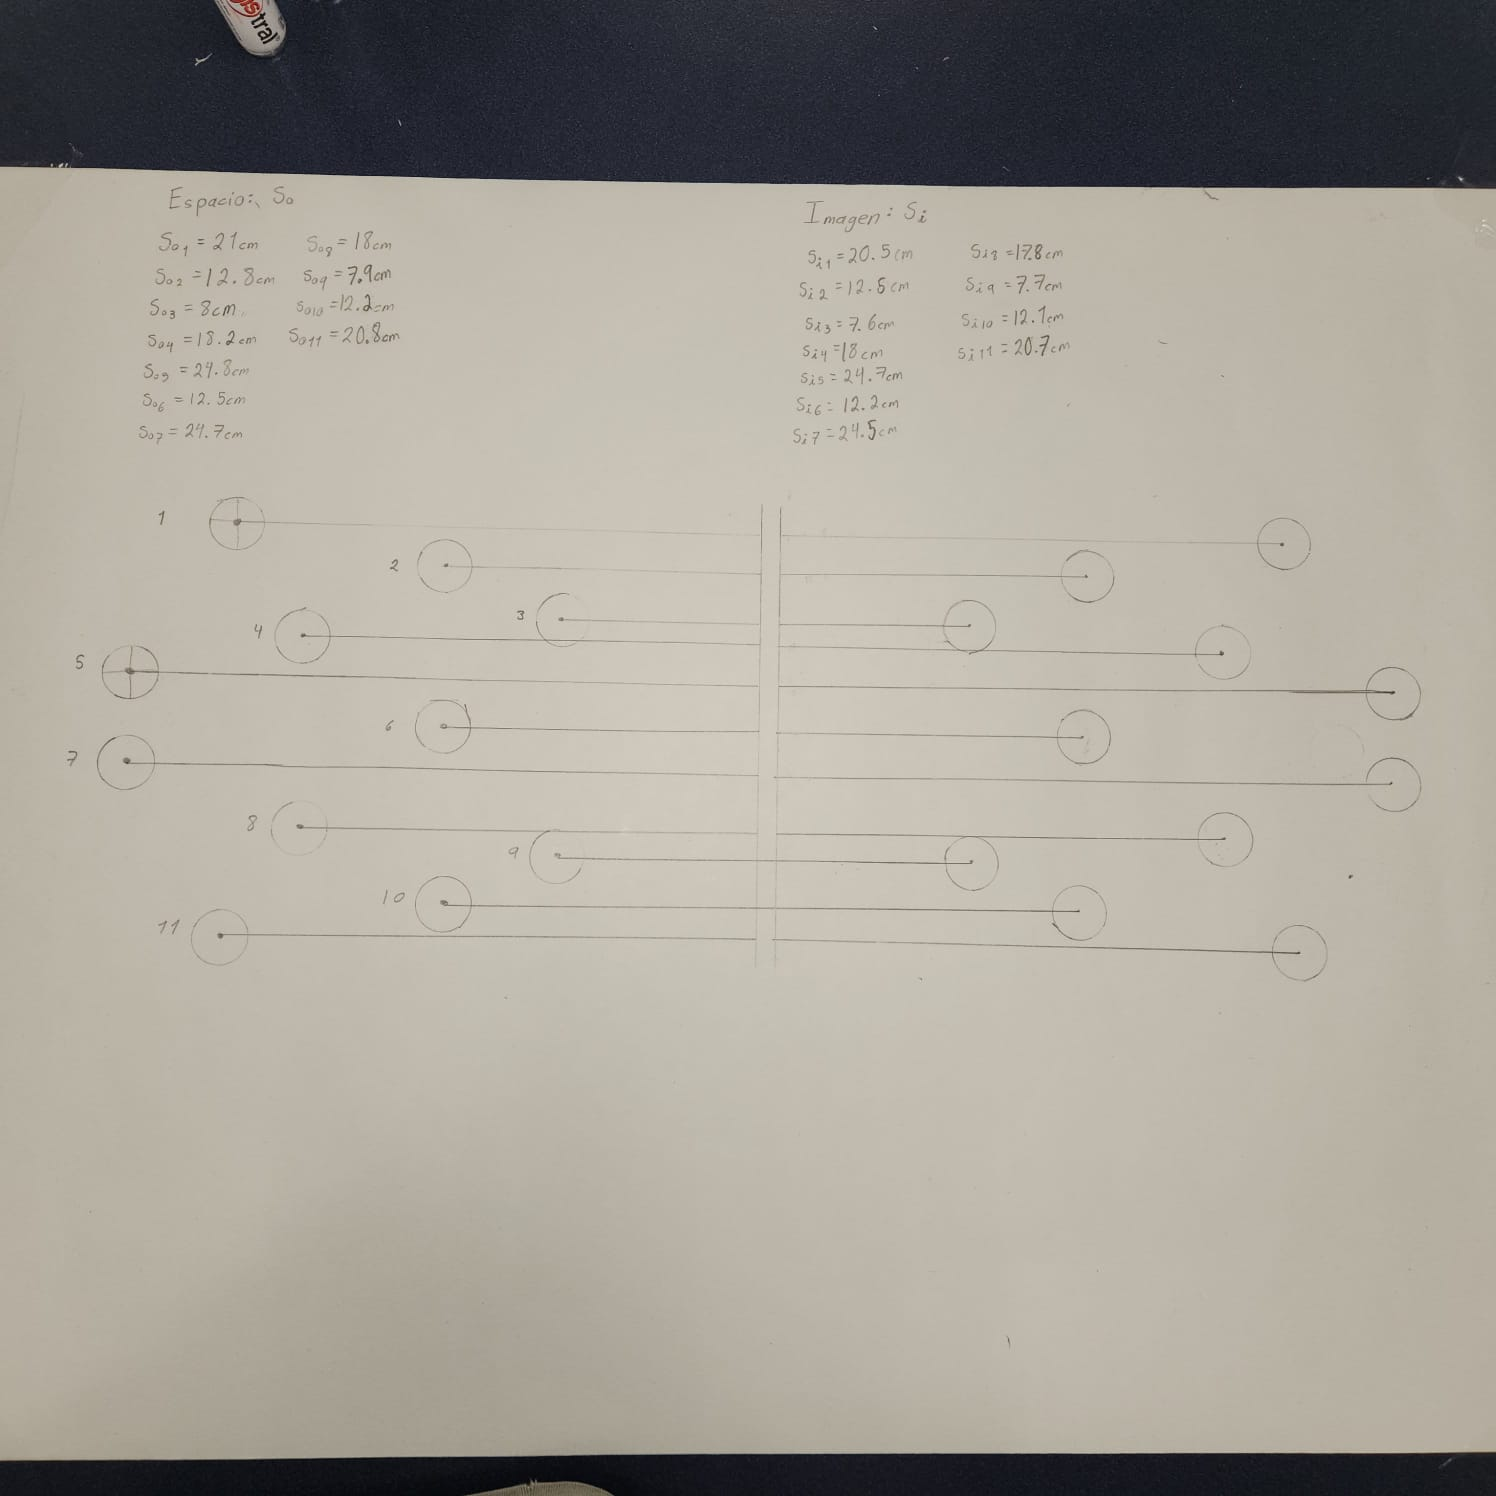
\includegraphics[width=\columnwidth]{trazo_espejo.jpg}
\captionof{figure}{Pliego con las once posiciones del objeto a la izquierda de la línea del espejo, sus imágenes a la derecha y las distancias medidas anotadas en la parte superior.}
\label{fig:trazo}
\end{center}
